% Für Bindekorrektur als optionales Argument "BCORfaktormitmaßeinheit", dann
% sieht auch Option "twoside" vernünftig aus
% Näheres zu "scrartcl" bzw. "scrreprt" und "scrbook" siehe KOMA-Skript Doku
\documentclass[12pt,a4paper,titlepage,headinclude,bibtotoc]{scrartcl}


%---- Allgemeine Layout Einstellungen ------------------------------------------

% Für Kopf und Fußzeilen, siehe auch KOMA-Skript Doku
\usepackage[komastyle]{scrpage2}
\pagestyle{scrheadings}
\automark[section]{chapter}
\setheadsepline{0.5pt}[\color{black}]

%keine Einrückung
\parindent0pt

%Einstellungen für Figuren- und Tabellenbeschriftungen
\setkomafont{captionlabel}{\sffamily\bfseries}
\setcapindent{0em}


%---- Weitere Pakete -----------------------------------------------------------
% Die Pakete sind alle in der TeX Live Distribution enthalten. Wichtige Adressen
% www.ctan.org, www.dante.de

% Sprachunterstützung
\usepackage[ngerman]{babel}

% Benutzung von Umlauten direkt im Text
% entweder "latin1" oder "utf8"
\usepackage[utf8]{inputenc}

% Pakete mit Mathesymbolen und zur Beseitigung von Schwächen der Mathe-Umgebung
\usepackage{latexsym,exscale,amssymb,amsmath}

% Weitere Symbole
\usepackage[nointegrals]{wasysym}
\usepackage{eurosym}

% Anderes Literaturverzeichnisformat
%\usepackage[square,sort&compress]{natbib}

% Für Farbe
\usepackage{color}

% Zur Graphikausgabe
%Beipiel: \includegraphics[width=\textwidth]{grafik.png}
\usepackage{graphicx}

% Text umfließt Graphiken und Tabellen
% Beispiel:
% \begin{wrapfigure}[Zeilenanzahl]{"l" oder "r"}{breite}
%   \centering
%   \includegraphics[width=...]{grafik}
%   \caption{Beschriftung} 
%   \label{fig:grafik}
% \end{wrapfigure}
\usepackage{wrapfig}

% Mehrere Abbildungen nebeneinander
% Beispiel:
% \begin{figure}[htb]
%   \centering
%   \subfigure[Beschriftung 1\label{fig:label1}]
%   {\includegraphics[width=0.49\textwidth]{grafik1}}
%   \hfill
%   \subfigure[Beschriftung 2\label{fig:label2}]
%   {\includegraphics[width=0.49\textwidth]{grafik2}}
%   \caption{Beschriftung allgemein}
%   \label{fig:label-gesamt}
% \end{figure}
\usepackage{subfigure}

% Caption neben Abbildung
% Beispiel:
% \sidecaptionvpos{figure}{"c" oder "t" oder "b"}
% \begin{SCfigure}[rel. Breite (normalerweise = 1)][hbt]
%   \centering
%   \includegraphics[width=0.5\textwidth]{grafik.png}
%   \caption{Beschreibung}
%   \label{fig:}
% \end{SCfigure}
\usepackage{sidecap}

% Befehl für "Entspricht"-Zeichen
\newcommand{\corresponds}{\ensuremath{\mathrel{\widehat{=}}}}

%Für chemische Formeln (von www.dante.de)
%% Anpassung an LaTeX(2e) von Bernd Raichle
\makeatletter
\DeclareRobustCommand{\chemical}[1]{%
  {\(\m@th
   \edef\resetfontdimens{\noexpand\)%
       \fontdimen16\textfont2=\the\fontdimen16\textfont2
       \fontdimen17\textfont2=\the\fontdimen17\textfont2\relax}%
   \fontdimen16\textfont2=2.7pt \fontdimen17\textfont2=2.7pt
   \mathrm{#1}%
   \resetfontdimens}}
\makeatother

%Si Einheiten
\usepackage{siunitx}

%c++ Code einbinden
\usepackage{listings}
\lstset{numbers=left, numberstyle=\tiny, numbersep=5pt}

%Differential
\newcommand{\dif}{\ensuremath{\mathrm{d}}}

%Boxen,etc.
\usepackage{fancybox}
\usepackage{empheq}

%Fußnoten auf gleiche Seite
\interfootnotelinepenalty=1000

%Dateien aus Unterverzeichnissen
\usepackage{import}              

\begin{document}

\begin{titlepage}
\centering
\textsc{\Large CWR 2 SoSe 2014, Fakultät für
  Physik,\\[1.5ex] Universität Göttingen}

\vspace*{4.2cm}

\rule{\textwidth}{1pt}\\[0.5cm]
{\huge \bfseries
  Projekt 65\\[1.5ex]
  Doppelpendel}\\[0.5cm]
\rule{\textwidth}{1pt}

\vspace*{3.0cm}

\begin{Large}
\begin{tabular}{lr}
 Bearbeiter:  &  Felix Kurtz\\
 E-Mail: &  felix.kurtz@stud.uni-goettingen.de\\
 Betreuer: & Burkhard Blobel \\
 Abgabe: & 18.08.2014\\
\end{tabular}
\end{Large}

\vspace*{0.8cm}
\begin{Large}
\fbox{
\begin{minipage}[t][2.5cm][t]{6cm}
Note:
\end{minipage}
}
\end{Large}

\end{titlepage}

\tableofcontents

\newpage

\section{Aufgabenstellung}
In dieser Hausarbeit stehen die Bewegungen eines Doppelpendels im Vordergrund.\\
\begin{figure}[!htb]
	\centering	
	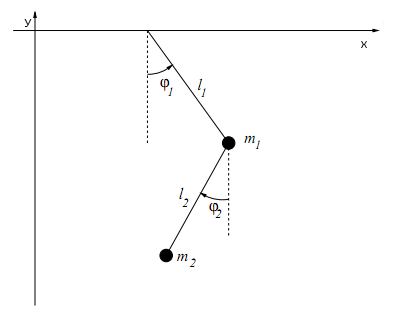
\includegraphics[scale=0.8]{doppelpendel.png}
	\caption{Doppelpendel mit wichtigen Größen \protect\footnotemark}
\end{figure}
\footnotetext{Quelle: http://me-lrt.de/img/vari-u05-2-doppelpendel.png}

Man kann es mit folgendem System gekoppelter Differentialgleichungen beschreiben.
\begin{align}
	Ml_1\ddot{\varphi}_1 + m_2l_2\ddot{\varphi}_2\cos\left(\varphi_1-\varphi_2\right) + m_2l_2\dot{\varphi}_2^2\sin\left(\varphi_1-\varphi_2\right) + Mg\sin\varphi_1 &= 0 \label{eq:bew1} \\
	m_2l_2\ddot{\varphi}_2 + m_2l_1\ddot{\varphi}_1\cos\left(\varphi_1-\varphi_2\right) - m_2l_1\dot{\varphi}_1^2\sin\left(\varphi_1-\varphi_2\right) + m_2g\sin\varphi_2&=0 \label{eq:bew2}
\end{align}
Dabei ist $M=m_1+m_2$.
Zuerst soll dieses System 2.Ordnung auf eines erster Ordnung zurückgeführt werden, um diese anschließend mittels Runge-Kutta-Verfahren 2. und 4.Ordnung numerisch zu integrieren.\\
Man fixiert $l_1=1\si{\meter}$ und $m_1=1\si{\kilo\gram}$ und variiert die Verhältnisse $l_2/l_1$ und $m_2/m_1$.
Für die Anfangsbedingungen $\varphi_1(0)=\frac{\pi}{4}$, $\dot{\varphi}_1=1 \frac{\si{rad}}{\si{\second}}$ und $\varphi_2(0)=\frac{\pi}{3}$, $\dot{\varphi}_2=1.5 \frac{\si{rad}}{\si{\second}}$ wird dann das Verhalten des Pendels untersucht.
Es soll die Bahn der beiden Massen geplottet werden sowie ihre Geschwindigkeiten in Abhängigkeit des Ortes.
Neben dem qualitativen Verhalten des Pendels sollen auch die beiden genutzten Integrationsverfahren hinsichtlich Geschwindigkeit und Genauigkeit getestet werden.

\section{System umschreiben}
Stellt man \eqref{eq:bew2} nach $\ddot{\varphi}_2$ um und setzt man dies in \eqref{eq:bew1} ein, kann diese Gleichung nach $\ddot{\varphi}_1$ aufgelöst werden. Analog stellt man \eqref{eq:bew2} nach $\ddot{\varphi}_1$ um und setzt dies in \eqref{eq:bew1} ein, um $\ddot{\varphi}_2$ zu erhalten. 
\begin{align}
	\ddot{\varphi}_1 &= -\left(m_2l_1\dot{\varphi}_1^2sc - m_2g\sin\varphi_2c + m_2l_2\dot{\varphi}_2^2s+Mg\sin\varphi_1 \right)/ \left(l_1M-l_1m_2c^2\right)\\
	\ddot{\varphi}_2 &= \left(Ml_1\dot{\varphi}_1^2s - Mg\sin\varphi_2 + m_2l_2\dot{\varphi}_2^2sc+Mg\sin\varphi_1c \right)/ \left(l_2M-l_2m_2c^2\right)
\end{align}
Hier ist $s=\sin\left(\varphi_1-\varphi_2\right)$ und $c=\cos\left(\varphi_1-\varphi_2\right)$.\\
Nun hängen die zweiten Ableitungen nicht mehr von der jeweils anderen zweiten Ableitung ab.
Substituiert man nun noch $\dot{\varphi}_1$ bsp. durch $\theta_1$ und analog $\dot{\varphi}_2$ durch $\theta_2$, sind diese 4 Gleichungen ein System erster Ordnung.
Dies kann nun numerisch gelöst werden. 

\section{Kartesische Koordinaten und Energie}
Aus den Winkeln und Seillängen lassen sich so die kartesischen Koordinaten berechnen:
\begin{align*}
	x_1 &= l_1\sin\varphi_1\\
	y_1 &= -l_1\cos\varphi_1\\	
	x_2 &= x_1+l_2\sin\varphi_2\\
	y_2 &= y_1-l_2\cos\varphi_2\\
\end{align*}
Leitet man diese ab, erhält man die Geschwindigkeiten.
\begin{align*}
	\dot{x}_1 &= l_1\cos\varphi_1 \cdot \dot{\varphi}_1\\
	\dot{y}_1 &= l_1\sin\varphi_1 \cdot \dot{\varphi}_1\\	
	\dot{x}_2 &= \dot{x}_1 + l_2\cos\varphi_2 \cdot \dot{\varphi}_2\\
	\dot{y}_2 &= \dot{y}_1 + l_2\sin\varphi_2 \cdot \dot{\varphi}_2\\
\end{align*}
Aus all diesen Werten kann die Gesamtenergie des Doppelpendels berechnet werden:
\begin{align*}
	E = E_{pot}+E_{kin} = m_1gy_1+m_2gy_2 + \frac{1}{2}m_1\left(\dot{x}_1^2+\dot{y}_1^2\right) + \frac{1}{2}m_2\left(\dot{x}_2^2+\dot{y}_2^2\right)
\end{align*}

\section{Programmaufbau}
Ich habe mich für den objektorientierten Ansatz entschieden.
So beschreibt die Klasse \textit{Doppelpendel} eben dieses. 
Sie hat folgende Attribute:
\begin{itemize}
	\item Massen und Längen	
	\item $\varphi_1$ und $\varphi_2$ sowie ihre ersten Ableitungen
	\item zugehörige kartesische Koordinaten - auch Geschwindigkeiten
	\item Energie - anfangs und aktuell
	\item Saltozähler
	\item Zeit
\end{itemize}
Die Berechnung der Energie dient der Beurteilung, wie gut die Trajektorie berechnet wurde, da sie konstant sein sollte.
Die Zählung der Saltos - also wenn die Winkel $82n+1)\pi$ überschreiten - habe ich hinzugefügt, um das Verhalten des Pendels einfacher beurteilen zu können, vor allem in Hinblick auf verschiedene Massen- und Längenverhältnisse.
So muss nicht jede Trajektorie angeschaut werden.\\
Der \textit{Konstruktor} setzt $m_1=1\si{\kilo\gram}$ und $l_1=1\si{\meter}$, da wir uns hier nur auf diesen Fall beschränken.
Da alle Attribute jedoch \textit{public} sind, könnte man diese beiden auch ändern.
Mit der Memberfunktion \textit{initialize} werden die restlichen Variablen gesetzt.
So kann diese öfters aufgerufen werden und das Doppelpendel mit neuen Anfangsbedingungen gestartet werden.\\
Berechnung der Trajektorie\\
Außerdem hat sie noch weitere Methoden:
\begin{itemize}
	\item $\ddot{\varphi}_1\left(\varphi_1, \dot{\varphi}_1,\varphi_2, \dot{\varphi}_2\right)$ und $\ddot{\varphi}_2\left(\varphi_1, \dot{\varphi}_1,\varphi_2, \dot{\varphi}_2\right)$
	\item Runge-Kutta 2. und 4.Ordnung	
	\item Berechnung der kartesischen Koordinaten und deren Ableitungen
	\item Berechnung der Gesamtenergie
\end{itemize}

Des Weiteren habe ich noch zwei Methoden implementiert, die den Abstand der Massen zwei verschiedener Doppelpendel zurückgibt.

\section{Vergleich der Integrationsverfahren}
Zwar ist Runge-Kutta 2.Ordnung mit gleicher Integrationsschrittweite schneller als der 4.Ordnung, aber auch ungenauer. 
Dies ist bei einem chaotischen System wie diesem unerwünscht.

\section{Entwicklung der Gesamtenergie}
Um die Genauigkeit des Integrationsverfahrens zu überprüfen, kann man sich die Gesamtenergie anschauen.
Diese sollte bekanntlich konstant sein.
In Abbildung ... ist die Energie gegen die Zeit aufgetragen.
Man erkennt, dass es Energiespitzen gibt. 
Die Gesamtenergie fällt jedoch in Fall A ungefähr auf das anfängliche Niveau zurück.
In Fall B klettert die Energie unaufhörlich, die Simulation ist also nur zu einem gewissen Grad brauchbar.

\section{Scan}
\begin{figure}[!htb]
	\centering
	\subimport*{Programm/}{salto1rk4.tex}
	\caption{Zahl der Überschläge der ersten Masse nach 20 Sekunden mitttels Runge-Kutta 4.Ordnung}
\end{figure}

\begin{figure}[!htb]
	\centering
	\subimport*{Programm/}{salto2rk4.tex}
	\caption{Zahl der Überschläge der zweiten Masse nach 20 Sekunden mitttels Runge-Kutta 4.Ordnung}
\end{figure}

\begin{figure}[!htb]
	\centering
	\subimport*{Programm/}{energie_rk4.tex}
	\caption{Energie nach 20 Sekunden mitttels Runge-Kutta 4.Ordnung}
\end{figure}

\begin{figure}[!htb]
	\centering
	\subimport*{Programm/}{energie0_rk4.tex}
	\caption{Anfangsenergie}
\end{figure}

\section{Trajektorien}

\begin{figure}[!htb]
	\centering
	\subimport*{Programm/}{trajektorie1.tex}
	\caption{$l_2=5.75\si{\meter}$, $m_2=7\si{\kilo\gram}$, 20 Sekunden, $\Delta t = 0.005 \si{\second}$}
\end{figure}

\begin{figure}[!htb]
	\centering
	\subimport*{Programm/}{trajektorie2.tex}
	\caption{$l_2=0.5\si{\meter}$, $m_2=0.05\si{\kilo\gram}$, 20 Sekunden, $\Delta t = 0.005 \si{\second}$}
\end{figure}

\begin{figure}[!htb]
	\centering
	\subimport*{Programm/}{trajektorie3.tex}
	\caption{$l_2=1\si{\meter}$, $m_2=1\si{\kilo\gram}$, 20 Sekunden, $\Delta t = 0.005 \si{\second}$}
\end{figure}

\begin{figure}[!htb]
	\centering
	\subimport*{Programm/}{trajektorie4.tex}
	\caption{$l_2=3\si{\meter}$, $m_2=0.6\si{\kilo\gram}$, 20 Sekunden, $\Delta t = 0.005 \si{\second}$}
\end{figure}

\begin{figure}[!htb]
	\centering
	\subimport*{Programm/}{trajektorie5.tex}
	\caption{$l_2=3\si{\meter}$, $m_2=0.6\si{\kilo\gram}$, 40 Sekunden, $\Delta t = 0.005 \si{\second}$}
\end{figure}

\section{Anhang}

\end{document}
